\chapter{Metryki}
\label{cha:metryki}
Podstawowymi miarami obrazującymi jakość uczenia sieci neuronowej jest dokładność (\textit{ang. accuracy}) oraz wartość funkcji kosztu (\textit{ang. loss value}).

Dokładność to procent prawidłowych klasyfikacji, zatem wyznaczenie tej wartości dla zbioru uczącego i testowego obrazuje jakość uczenia. Można również zaobserwować, czy jest różnica między tym, jak sieć radzi sobie z danymi, które już zna i tymi, które widzi po raz pierwszy.

Celem procesu uczenia jest minimalizacja funkcji kosztu, zatem im niższa jej wartość, tym lepsza jest nasza sieć. Gdy wartość tej funkcji zaczyna rosnąć, mamy do czynienia z problemem przeuczenia.

\section{Porównanie metryk}
\label{cha:wyniki}
Pierwszy analizowany model ma następujące parametry:
\begin{itemize}
  \item Optymalizator: \textbf{Adam}
  \item Wskaźnik uczenia: \textbf{0,01}
  \item Wymiary warstwy ukrytej: \textbf{16}
  \item Liczba epok: \textbf{20}
 \end{itemize}
 
 Jak widać na wykresie 7.1, występuje duża rozbieżność między dokładnością zbioru uczącego a dokładnością zbioru treningowego i testowego. W każdym z analizowanych podczas badań przypadków ta różnica była podobna lub nawet większa. Ani razu podczas przeprowadzanych badań nie udało się osiągnąć w zbiorze testowym dokładności większej niż 78\%.m. Powodem takiej sytuacji może być zjawisko nadmiernego dopasowania, gdzie model uczy się konkretnych reguł, których nie jest w stanie rozszerzyć poza zbiór uczący. Iną przyczyną może być zbyt mała ilość danych uczących. Ta opcja jest bardziej prawdopodobna, gdyż dokładność w zbiorze testowym stabilizuje się już po kilku epokach i ma bardzo zbliżone wartości niezależnie od wyboru parametrów (dlatego w rozdziale szóstym wartość ta nie została uwzględniona w tabelach porównawczych). Końcowa dokładność klasyfikacji zbioru uczącego to 96,77\%, jest to również wartość nalepsza ze wszystkich epok. Dla zbioru testowego dokładność po dwudziestu epokach wynosi 76,6\%, natomiast najlepszą wartość wynoszącą 78\% uzyskano w ósmej epoce.
 
 \label{sec:etykiety}
\begin{figure}[H]
    \centering
    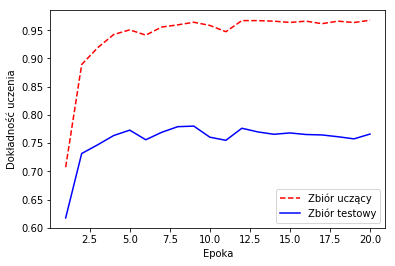
\includegraphics[clip]{accuracy16.png}
    \caption{Porównanie dokładności uczenia dla zbioru treningowego i testowego.}
\end{figure}


 \label{sec:etykiety}
\begin{figure}[H]
    \centering
    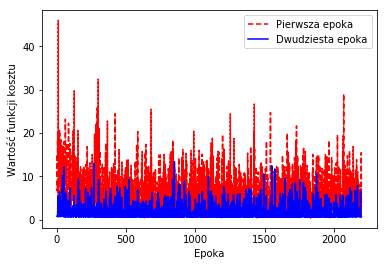
\includegraphics[clip]{compare-loss16.png}
    \caption{Porównanie wartości funkcji kosztu dla pierwszej i dwudziestej epoki uczenia.}
\end{figure}

Wykres 7.2 obrazuje różnicę w wartościach funkcji kosztu osiąganych w pierwszej i ostatniej epoce treningu. Widzimy, że proces uczenia przebiega prawidłowo \textendash \ średni koszt w pierwszej epoce wynosi 6,12, natomiast w dwudziestej 1,63. 

Wartość funkcji kosztu dla danych testowych szybko się stabilizuje osiągając minimum, co pokazuje wykres 7.3. Średni koszt w ostatniej epoce wynosi 0,69. 

 \label{sec:etykiety}
\begin{figure}[H]
    \centering
    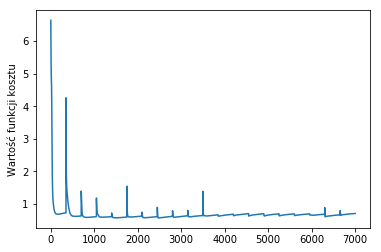
\includegraphics[clip]{test-loss16.png}
    \caption{Wartość funkcji kosztu dla zbioru testowego.}
\end{figure}

Dla porównania przeanalizowano również wykresy modelu z następującymi parametrami:
\begin{itemize}
  \item Optymalizator: \textbf{Adam}
  \item Wskaźnik uczenia: \textbf{0,01}
  \item Wymiary warstwy ukrytej: \textbf{32}
  \item Liczba epok: \textbf{70}
 \end{itemize}
 
 Jak widać na wykresie 7.4, dokładność klasyfikacji zbioru uczącego osiąga stabilność po ósmej epoce, a wartości są zbliżone do tych z wykresu 7.1. Wynik uzyskany po siedemdziesięciu epokach to 96,8\%, natomiast najlepsza uzyskana wartość to 97,8\%. 
 
  \label{sec:etykiety}
\begin{figure}[H]
    \centering
    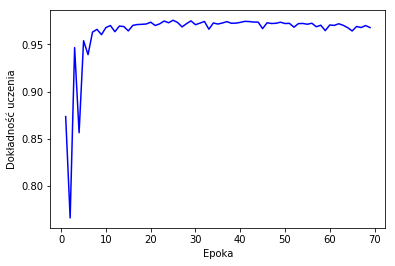
\includegraphics[clip]{train_acc.png}
    \caption{Dokładność uczenia dla zbioru treningowego.}
\end{figure}

 \label{sec:etykiety}
\begin{figure}[H]
    \centering
    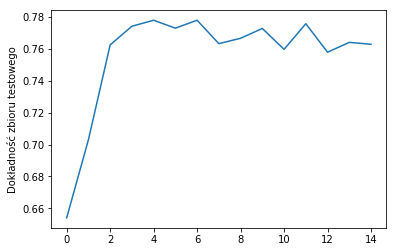
\includegraphics[clip]{test_acc.png}
    \caption{Dokładność uczenia dla zbioru testowego.}
\end{figure}

Dokładność dopasowań w zbiorze testowym (wykres 7.5) po siedemdziesięciu epokach wynosi 76,4\%, natomiast najlepsza uzyskana to 77,79\%. 

Zastanawiający jest przebieg wykresu 7.6, przedstawiającego zmianę wartości funkcji kosztu dla danych testowych. Wartość ta rośnie w miarę uczenia, co wskazuje na to, że mamy do czynienia z przeuczeniem. Jednak na wykresie 7.5 widzimy, że dokładność uczenia wraz z kolejnymi epokami utrzymuje się na tym samym poziomie. Może to oznaczać, że mimo iż model nie popełnia nowych błędów, to coraz bardziej utwierdza się w błędnych dopasowaniach.


 \label{sec:etykiety}
\begin{figure}[H]
    \centering
    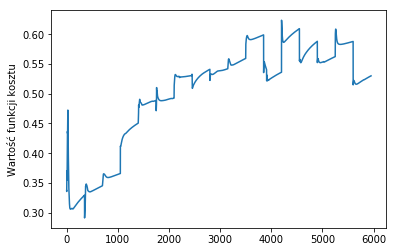
\includegraphics[clip]{test_loss.png}
    \caption{Wartość funkcji kosztu dla zbioru testowego.}
\end{figure}

Dla zbioru uczącego wartość funkcji kosztu w ostatniej epoce jest znacznie niższa niż w siedemdziesiątej (co przedstawia wykres 7.7), więc w tym przypadku sieć zachowuje się prawidłowo.

Do dalszej analizy metryk w tym rozdziale oraz przypadków w rozdziale 8 wybrano drugą z opisywanych w tym podpunkcie sieci.

 \label{sec:etykiety}
\begin{figure}[H]
    \centering
    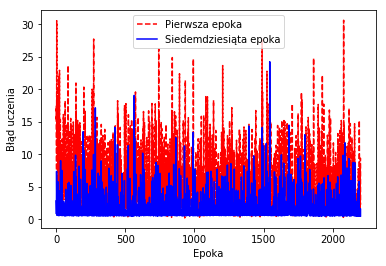
\includegraphics[clip]{epoch1vs70.png}
    \caption{Porównanie wartości funkcji kosztu dla pierwszej i siedemdziesiątej epoki uczenia.}
\end{figure}
 
\section{Raport klasyfikacji}
\label{cha:wyniki}

\begin{table}[H]
\centering
\begin{tabular}{|lllll|}
\hline
\multicolumn{1}{|l|}{\textbf{}}               & \multicolumn{1}{c|}{\textbf{precyzja}} & \multicolumn{1}{c|}{\textbf{czułość}} & \multicolumn{1}{l|}{\textbf{miara F-1}} & \textbf{liczba wystąpień} \\ \hline
\multicolumn{1}{|l|}{\textbf{neutralne}}      & \multicolumn{1}{c|}{0,84}              & \multicolumn{1}{c|}{0,90}         & \multicolumn{1}{l|}{0,87}               & 3666                      \\ \hline
\multicolumn{1}{|l|}{\textbf{pozytywne}}      & \multicolumn{1}{c|}{0.70}              & \multicolumn{1}{c|}{0,40}         & \multicolumn{1}{l|}{0,51}               & 1016                      \\ \hline
\multicolumn{1}{|l|}{\textbf{negatywne}}      & \multicolumn{1}{c|}{0,29}              & \multicolumn{1}{l|}{0,41}         & \multicolumn{1}{l|}{0,34}               & 365                       \\ \hline
\end{tabular}
\caption{Raport klasyfikacji modelu po 70 epokach uczenia.}
\label{table:bf-sa}
\end{table}

Precyzja to stosunek liczby prawdziwie pozytywnych dopasowań do wszystkich dopasowań. Jak widać sieć radzi sobie dobrze z dopasowaniem etykiet neutralnych i całkiem dobrze rozpoznaje wydźwięk pozytywny. Natomiast w przypadku etykiet negatywnych mamy bardzo niską precyzję, widać, że w większości przypadków sieć źle dopasowuje wydźwięk negatywny.

Czułość to stosunek liczby dopasowań prawdziwie pozytywnych do ogólnej liczby możliwych dopasowań. W tym przypadku widzimy, że tylko 40\% etykiet pozytywnych zostało dopasowanych. 

Miara F-1 jest średnią harmoniczną precyzji i czułości, zatem obrazuje ogólną jakość modelu. Widzimy, że dla etykiet neutralnych klasyfikacja przebiega prawidłowo, natomiast dla etykiet pozytywnych i negatywnych nie działa zbyt dobrze. 

Powodem takich wyników może być znaczna przewaga etykiet neutralnych w zbiorze uczącym, dzięki czemu sieć mogła się lepiej wyuczyć związanych z nimi zależności. Najmniej liczne były etykiety negatywne, co przekłada się na wyniki klasyfikacji. Dokładną liczbę dopasowań konkretnych etykiet do danych testowych obrazuje macierz konfuzji z rys. 7.8.


\label{sec:etykiety}
\begin{figure}[H]
    \centering
    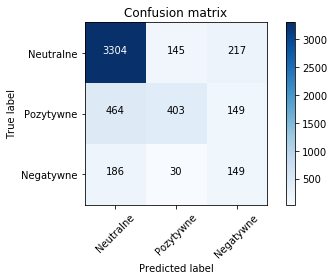
\includegraphics[clip]{conmat67.png}
    \caption{Macierz konfuzji modelu po 70 epokach uczenia.}
\end{figure}


